\documentclass[11pt]{article}
\usepackage[utf8]{inputenc}
\usepackage[english]{babel}
%\usepackage{fancyhdr}
%\usepackage{dsfont} %eins als neutrales element
%\renewcommand{\rmdefault}{ppl}
%\usepackage{caption,chngcntr}
%!TeX spellcheck = en_US 
\usepackage{lmodern}


\usepackage{hyperref}
\usepackage{mathrsfs}
\usepackage{enumitem} 
\usepackage{paralist}
\usepackage[ 
left=2.5cm,    
right=2.5cm,
top=2cm,
bottom=2cm,
]{geometry}

\usepackage[labelfont={},font={footnotesize}]{caption}

\renewcommand{\figurename}{Fig.}
\renewcommand{\tablename}{Tab.}

%\numberwithin{table}{section}
%\numberwithin{figure}{section}
%\numberwithin{equation}{section}

\usepackage{array}
\newcolumntype{L}[1]{>{\raggedright\let\newline\\\arraybackslash\hspace{0pt}}m{#1}}
\newcolumntype{C}[1]{>{\centering\let\newline\\\arraybackslash\hspace{0pt}}m{#1}}
\newcolumntype{R}[1]{>{\raggedleft\let\newline\\\arraybackslash\hspace{0pt}}m{#1}}

\usepackage{fancybox} 
\usepackage[T1]{fontenc} 

\usepackage[arrow, matrix, curve]{xy}
\usepackage{amsthm}
\usepackage{paralist}
%\usepackage{graphicx} 
%\usepackage{tabularx}
\usepackage{amssymb}
\usepackage{amsmath}


\usepackage{setspace}	
\setstretch{1.2}
\usepackage{natbib}
\bibliographystyle{apalike}

%tikz
\usepackage{tikz}
\usetikzlibrary{shapes.geometric, arrows}
\usetikzlibrary{arrows, arrows.meta, calc, positioning, quotes, shapes}
\usetikzlibrary{automata,positioning}
\usetikzlibrary{positioning, arrows}
\usetikzlibrary{decorations.pathmorphing}
\usetikzlibrary{calc}
\usetikzlibrary{matrix}
\usetikzlibrary {arrows.meta} 

\usepackage{float}
\setlength{\parindent}{0pt} 

\definecolor{madrid}{rgb}{0.2,0.2,0.8}
\definecolor{darkgreen}{rgb}{0.2,0.6,0.2}
\definecolor{darkred}{rgb}{0.8,0.2,0.4}
\definecolor{orange}{rgb}{0.9,0.4,0.0}
\definecolor{lila}{rgb}{0.5,0,0.5}
\definecolor{gray}{rgb}{0.85,0.85,0.85}



%\theoremstyle{definition}
%\newtheorem{theorem}{Theorem}
%\newtheorem{definition}{Definition}
%\usepackage{varioref}


\begin{document}
	
		\begin{figure}[H]
			\small
			\fontfamily{lmss}\selectfont
			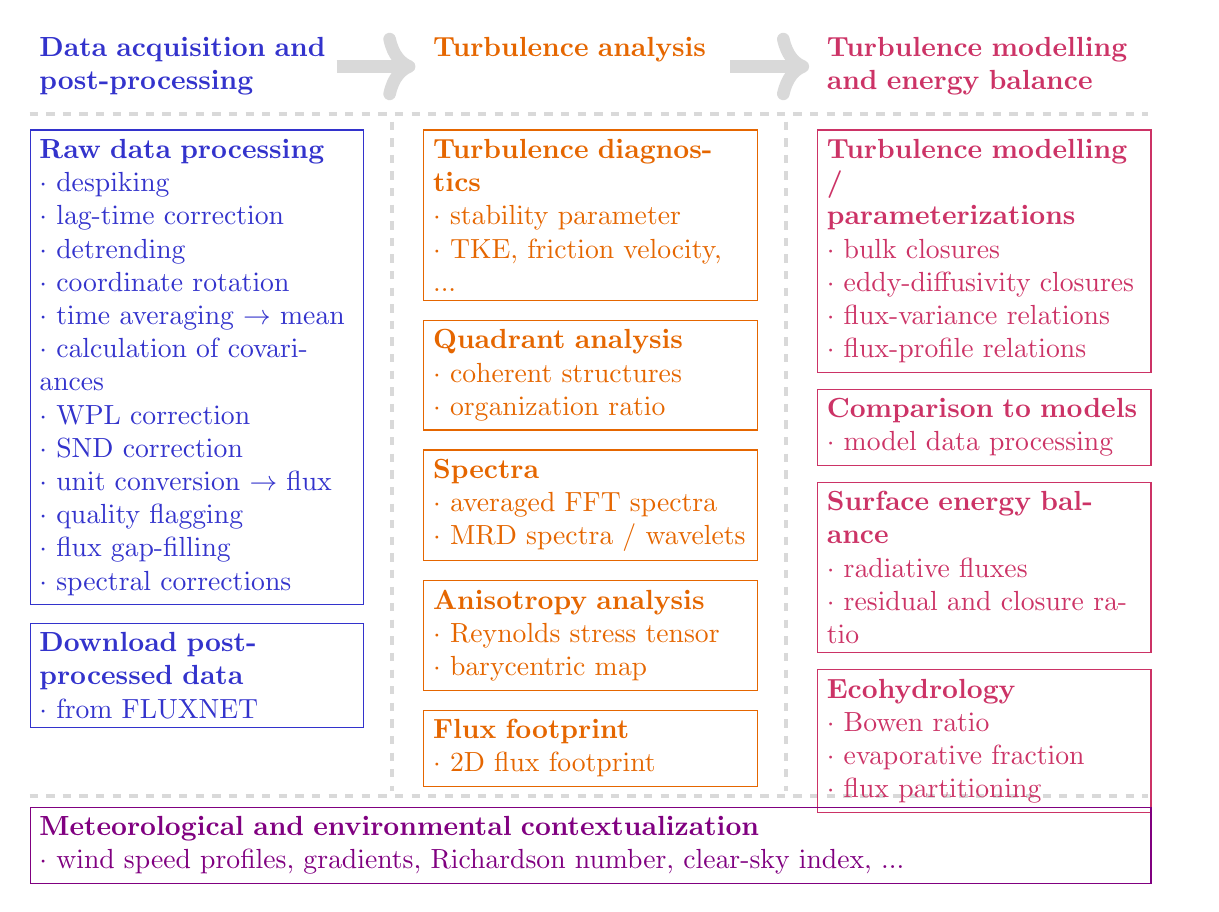
\begin{tikzpicture}
				\node(data) [text width = 4cm,madrid,anchor=north west] at (0,0) { \textbf{Data acquisition and post-processing}} ;
				\node(analysis) [text width = 4cm, orange,anchor=north west] at (5,0) { \textbf{Turbulence analysis} };
				\node(application) [text width = 4.5cm,darkred,anchor=north west] at (10,0) { \textbf{Turbulence modelling and energy balance} };
				
				%----------------------------------------------------------------
				\draw [arrows = {-Computer Modern Rightarrow[line cap=round]},gray,line width=1.6mm]
				(3.9,-0.5) -- (4.9,-0.5);
				\draw [arrows = {-Computer Modern Rightarrow[line cap=round]},gray,line width=1.6mm]
				(8.9,-0.5) -- (9.9,-0.5);
				
				\draw [gray,line width=0.5mm,dashed]
				(4.6,-1.2) -- (4.6,-9.7);
				\draw [gray,line width=0.5mm,dashed]
				(9.6,-1.2) -- (9.6,-9.7);
				\draw [gray,line width=0.5mm,dashed]
				(0,-1.1) -- (14.2,-1.1);
				\draw [gray,line width=0.5mm,dashed]
				(0,-9.77) -- (14.2,-9.77);
				
				%--------------------------------------------------------------------
				\node(raw) [text width = 4cm,madrid,draw,anchor=north west] at (0,-1.3) { \textbf{Raw data processing} \\
				$\cdot$ despiking \\
				$\cdot$ lag-time correction \\
				$\cdot$ detrending \\
				$\cdot$ coordinate rotation \\
				$\cdot$ time averaging $\rightarrow$ mean \\
				$\cdot$ calculation of covariances \\
				$\cdot$ WPL correction \\
				$\cdot$ SND correction \\
				$\cdot$ unit conversion $\rightarrow$ flux \\
				$\cdot$ quality flagging \\
				$\cdot$ flux gap-filling \\
				$\cdot$ spectral corrections
				} ;
				
				\node(download) [below=0.22cm of raw, text width = 4cm,madrid,draw]  { \textbf{Download post-processed data} \\
					$\cdot$ from FLUXNET
				} ;
				
				
				%---------------------------------------------------------------------
				\node(diagnostics) [text width = 4cm,orange,draw,anchor=north west]  at (5,-1.3) { \textbf{Turbulence diagnostics} \\
				$\cdot$ stability parameter \\
				$\cdot$ TKE, friction velocity, ...  
				} ;
			   \node(qa) [text width = 4cm,orange,draw,below=0.24cm of diagnostics] { \textbf{Quadrant analysis} \\
			   	$\cdot$ coherent structures \\
			   	$\cdot$ organization ratio 
			   } ;
				\node(spectra) [text width = 4cm,orange,draw,below=0.24cm of qa] { \textbf{Spectra} \\
					$\cdot$ averaged FFT spectra\\
					$\cdot$ MRD spectra / wavelets
				} ;
				\node(aniso) [text width = 4cm,orange,draw,below=0.24cm of spectra] { \textbf{Anisotropy analysis} \\
					$\cdot$ Reynolds stress tensor\\
					%$\cdot$ turbulence anisotropy \\
					$\cdot$ barycentric map
				} ;
				\node(footprint) [text width = 4cm,orange,draw,below=0.24cm of aniso] { \textbf{Flux footprint} \\
					$\cdot$ 2D flux footprint
				} ;
			
				%---------------------------------------------------------------
				
				\node(param) [text width = 4cm,darkred,draw,anchor=north west]  at (10,-1.3) { \textbf{Turbulence modelling / \\ parameterizations} \\
					$\cdot$ bulk closures  \\
					$\cdot$ eddy-diffusivity closures \\
					$\cdot$ flux-variance relations \\  
					$\cdot$ flux-profile relations
				} ;
				\node(comp) [text width = 4cm,darkred,draw,below=0.2cm of param] { \textbf{Comparison to models\\}
					$\cdot$ model data processing 
				} ;
				\node(seb) [text width = 4cm,darkred,draw,below=0.2cm of comp] { \textbf{Surface energy balance} \\
					$\cdot$ radiative fluxes \\
					$\cdot$ residual and closure ratio
				} ;
				\node(hyrdo) [text width = 4cm,darkred,draw,below=0.2cm of seb] { \textbf{Ecohydrology} \\
					$\cdot$ Bowen ratio \\
					$\cdot$ evaporative fraction\\
					$\cdot$ flux partitioning
				} ;
			
			
				%----------------------------------------------------------
			 	\node(meteo) [text width = 14cm,lila,anchor=north west,draw] at (0,-9.9) { \textbf{Meteorological and environmental contextualization} \\
			 	$\cdot$ wind speed profiles, gradients, Richardson number, clear-sky index, ...} ;

			
				%\draw[->, >=stealth',line width=1.5pt,text width=5cm, align=left] (start) -- (rans) node[midway,right] {\textbf{apply}: \\Reynolds average \\ Boussinesq approximation\\hydrostatic approximation} ;	
				
			\end{tikzpicture}
			\centering

		\end{figure}
	
	
	
	%%%%%%%%%%%%%%%%%%%%%%%%%%%%%%%%%%%%%%%%%%%%%%%%%%%%%%%%%%%%%%
	%%%%%%%%%%%%%%%%%%%%%%%%%%%%%%%%%%%%%%%%%%%%%%%%%%%%%%%%%%%%%%
	
	\newpage
	\begin{figure}[H]
		\small
		\fontfamily{lmss}\selectfont
		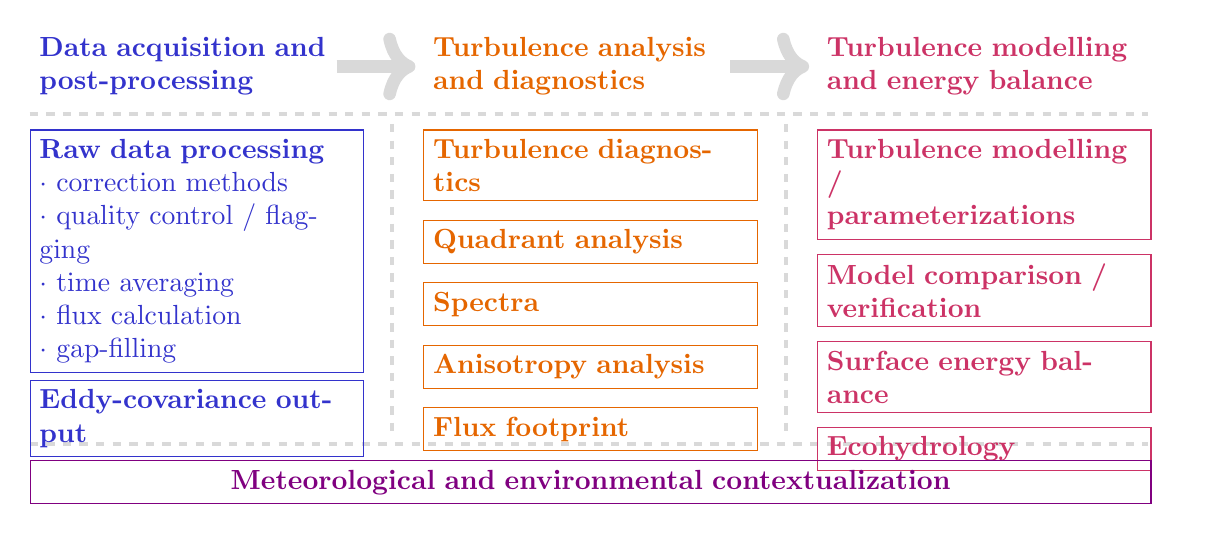
\begin{tikzpicture}
			\node(data) [text width = 4cm,madrid,anchor=north west] at (0,0) { \textbf{Data acquisition and post-processing}} ;
			\node(analysis) [text width = 4cm, orange,anchor=north west] at (5,0) { \textbf{Turbulence analysis \\ and diagnostics} };
			\node(application) [text width = 4.5cm,darkred,anchor=north west] at (10,0) { \textbf{Turbulence modelling and energy balance} };
			
			%----------------------------------------------------------------
			\draw [arrows = {-Computer Modern Rightarrow[line cap=round]},gray,line width=1.6mm]
			(3.9,-0.5) -- (4.9,-0.5);
			\draw [arrows = {-Computer Modern Rightarrow[line cap=round]},gray,line width=1.6mm]
			(8.9,-0.5) -- (9.9,-0.5);
			
			\draw [gray,line width=0.5mm,dashed]
			(4.6,-1.23) -- (4.6,-5.2);
			\draw [gray,line width=0.5mm,dashed]
			(9.6,-1.23) -- (9.6,-5.2);
			\draw [gray,line width=0.5mm,dashed]
			(0,-1.1) -- (14.2,-1.1);
			\draw [gray,line width=0.5mm,dashed]
			(0,-5.3) -- (14.2,-5.3);
			
			%--------------------------------------------------------------------
			\node(raw) [text width = 4cm,madrid,draw,anchor=north west] at (0,-1.3) { \textbf{Raw data processing } \\
				$\cdot$ correction methods \\
				$\cdot$ quality control / flagging \\
				$\cdot$ time averaging \\
				$\cdot$ flux calculation \\
				$\cdot$ gap-filling
				
%				$\cdot$ despiking \\
%				$\cdot$ lag-time correction \\
%				$\cdot$ detrending \\
%				$\cdot$ coordinate rotation \\
%				$\cdot$ time averaging $\rightarrow$ mean \\
%				$\cdot$ calculation of covariances \\
%				$\cdot$ WPL correction \\
%				$\cdot$ SND correction \\
%				$\cdot$ unit conversion $\rightarrow$ flux \\
%				$\cdot$ quality flagging \\
%				$\cdot$ flux gap-filling \\
%				$\cdot$ spectral corrections
			} ;
			
			\node(download) [below=0.09cm of raw, text width = 4cm,madrid,draw]  { \textbf{Eddy-covariance output} \\
%				$\cdot$ from FLUXNET
			} ;
			
			
			%---------------------------------------------------------------------
			\node(diagnostics) [text width = 4cm,orange,draw,anchor=north west]  at (5,-1.3) { \textbf{Turbulence diagnostics} \\
%				$\cdot$ stability parameter \\
%				$\cdot$ TKE, friction velocity, ...  
			} ;
			\node(qa) [text width = 4cm,orange,draw,below=0.233cm of diagnostics] { \textbf{Quadrant analysis} \\
%				$\cdot$ coherent structures \\
%				$\cdot$ organization ratio 
			} ;
			\node(spectra) [text width = 4cm,orange,draw,below=0.233cm of qa] { \textbf{Spectra} \\
%				$\cdot$ averaged FFT spectra\\
%				$\cdot$ MRD spectra / wavelets
			} ;
			\node(aniso) [text width = 4cm,orange,draw,below=0.233cm of spectra] { \textbf{Anisotropy analysis} \\
%				$\cdot$ Reynolds stress tensor\\
%				%$\cdot$ turbulence anisotropy \\
%				$\cdot$ barycentric map
			} ;
			\node(footprint) [text width = 4cm,orange,draw,below=0.233cm of aniso] { \textbf{Flux footprint} \\
%				$\cdot$ 2D flux footprint
			} ;
			
			%---------------------------------------------------------------
			
			\node(param) [text width = 4cm,darkred,draw,anchor=north west]  at (10,-1.3) { \textbf{Turbulence modelling / \\ parameterizations} \\
%				$\cdot$ bulk closures  \\
%				$\cdot$ eddy-diffusivity closures \\
%				$\cdot$ flux-variance relations \\  
%				$\cdot$ flux-profile relations
			} ;
			\node(comp) [text width = 4cm,darkred,draw,below=0.175cm of param] { \textbf{Model comparison / \\ verification\\}
%				$\cdot$ model data processing 
			} ;
			\node(seb) [text width = 4cm,darkred,draw,below=0.175cm of comp] { \textbf{Surface energy balance} \\
%				$\cdot$ radiative fluxes \\
%				$\cdot$ residual and closure ratio
			} ;
			\node(hyrdo) [text width = 4cm,darkred,draw,below=0.175cm of seb] { \textbf{Ecohydrology} \\
%				$\cdot$ Bowen ratio \\
%				$\cdot$ evaporative fraction\\
%				$\cdot$ flux partitioning
			} ;
			
			
			%----------------------------------------------------------
			\node(meteo) [text width = 14cm,lila,anchor=north west,draw,align=center] at (0,-5.5) { \textbf{Meteorological and environmental contextualization} \\
%				$\cdot$ wind speed profiles, gradients, Richardson number, clear-sky index, ...
			} ;
			
			
			%\draw[->, >=stealth',line width=1.5pt,text width=5cm, align=left] (start) -- (rans) node[midway,right] {\textbf{apply}: \\Reynolds average \\ Boussinesq approximation\\hydrostatic approximation} ;	
			
		\end{tikzpicture}
		\centering
		
	\end{figure}




\vspace{2cm}
\begin{figure}[H]
	\small
	\fontfamily{lmss}\selectfont
	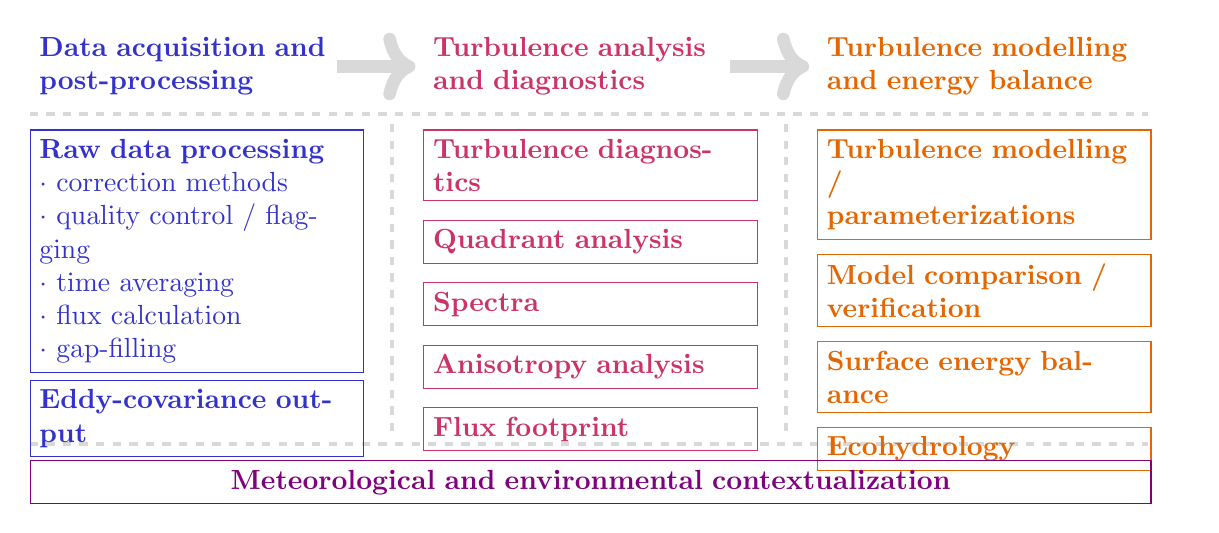
\begin{tikzpicture}
		\node(data) [text width = 4cm,madrid,anchor=north west] at (0,0) { \textbf{Data acquisition and post-processing}} ;
		\node(analysis) [text width = 4cm, darkred,anchor=north west] at (5,0) { \textbf{Turbulence analysis \\ and diagnostics} };
		\node(application) [text width = 4.5cm,orange,anchor=north west] at (10,0) { \textbf{Turbulence modelling \\ and energy balance} };
		
		%----------------------------------------------------------------
		\draw [arrows = {-Computer Modern Rightarrow[line cap=round]},gray,line width=1.6mm]
		(3.9,-0.5) -- (4.9,-0.5);
		\draw [arrows = {-Computer Modern Rightarrow[line cap=round]},gray,line width=1.6mm]
		(8.9,-0.5) -- (9.9,-0.5);
		
		\draw [gray,line width=0.5mm,dashed]
		(4.6,-1.23) -- (4.6,-5.2);
		\draw [gray,line width=0.5mm,dashed]
		(9.6,-1.23) -- (9.6,-5.2);
		\draw [gray,line width=0.5mm,dashed]
		(0,-1.1) -- (14.2,-1.1);
		\draw [gray,line width=0.5mm,dashed]
		(0,-5.3) -- (14.2,-5.3);
		
		%--------------------------------------------------------------------
		\node(raw) [text width = 4cm,madrid,draw,anchor=north west] at (0,-1.3) { \textbf{Raw data processing } \\
			$\cdot$ correction methods \\
			$\cdot$ quality control / flagging \\
			$\cdot$ time averaging \\
			$\cdot$ flux calculation \\
			$\cdot$ gap-filling
			
			%				$\cdot$ despiking \\
			%				$\cdot$ lag-time correction \\
			%				$\cdot$ detrending \\
			%				$\cdot$ coordinate rotation \\
			%				$\cdot$ time averaging $\rightarrow$ mean \\
			%				$\cdot$ calculation of covariances \\
			%				$\cdot$ WPL correction \\
			%				$\cdot$ SND correction \\
			%				$\cdot$ unit conversion $\rightarrow$ flux \\
			%				$\cdot$ quality flagging \\
			%				$\cdot$ flux gap-filling \\
			%				$\cdot$ spectral corrections
		} ;
		
		\node(download) [below=0.09cm of raw, text width = 4cm,madrid,draw]  { \textbf{Eddy-covariance output} \\
			%				$\cdot$ from FLUXNET
		} ;
		
		
		%---------------------------------------------------------------------
		\node(diagnostics) [text width = 4cm,darkred,draw,anchor=north west]  at (5,-1.3) { \textbf{Turbulence diagnostics} \\
			%				$\cdot$ stability parameter \\
			%				$\cdot$ TKE, friction velocity, ...  
		} ;
		\node(qa) [text width = 4cm,darkred,draw,below=0.233cm of diagnostics] { \textbf{Quadrant analysis} \\
			%				$\cdot$ coherent structures \\
			%				$\cdot$ organization ratio 
		} ;
		\node(spectra) [text width = 4cm,darkred,draw,below=0.233cm of qa] { \textbf{Spectra} \\
			%				$\cdot$ averaged FFT spectra\\
			%				$\cdot$ MRD spectra / wavelets
		} ;
		\node(aniso) [text width = 4cm,darkred,draw,below=0.233cm of spectra] { \textbf{Anisotropy analysis} \\
			%				$\cdot$ Reynolds stress tensor\\
			%				%$\cdot$ turbulence anisotropy \\
			%				$\cdot$ barycentric map
		} ;
		\node(footprint) [text width = 4cm,darkred,draw,below=0.233cm of aniso] { \textbf{Flux footprint} \\
			%				$\cdot$ 2D flux footprint
		} ;
		
		%---------------------------------------------------------------
		
		\node(param) [text width = 4cm,orange,draw,anchor=north west]  at (10,-1.3) { \textbf{Turbulence modelling / \\ parameterizations} \\
			%				$\cdot$ bulk closures  \\
			%				$\cdot$ eddy-diffusivity closures \\
			%				$\cdot$ flux-variance relations \\  
			%				$\cdot$ flux-profile relations
		} ;
		\node(comp) [text width = 4cm,orange,draw,below=0.175cm of param] { \textbf{Model comparison / \\ verification\\}
			%				$\cdot$ model data processing 
		} ;
		\node(seb) [text width = 4cm,orange,draw,below=0.175cm of comp] { \textbf{Surface energy balance} \\
			%				$\cdot$ radiative fluxes \\
			%				$\cdot$ residual and closure ratio
		} ;
		\node(hyrdo) [text width = 4cm,orange,draw,below=0.175cm of seb] { \textbf{Ecohydrology} \\
			%				$\cdot$ Bowen ratio \\
			%				$\cdot$ evaporative fraction\\
			%				$\cdot$ flux partitioning
		} ;
		
		
		%----------------------------------------------------------
		\node(meteo) [text width = 14cm,lila,anchor=north west,draw,align=center] at (0,-5.5) { \textbf{Meteorological and environmental contextualization} \\
			%				$\cdot$ wind speed profiles, gradients, Richardson number, clear-sky index, ...
		} ;
		
		
		%\draw[->, >=stealth',line width=1.5pt,text width=5cm, align=left] (start) -- (rans) node[midway,right] {\textbf{apply}: \\Reynolds average \\ Boussinesq approximation\\hydrostatic approximation} ;	
		
	\end{tikzpicture}
	\centering
	
\end{figure}






\vspace{2cm}
\begin{figure}[H]
	\small
	\fontfamily{lmss}\selectfont
	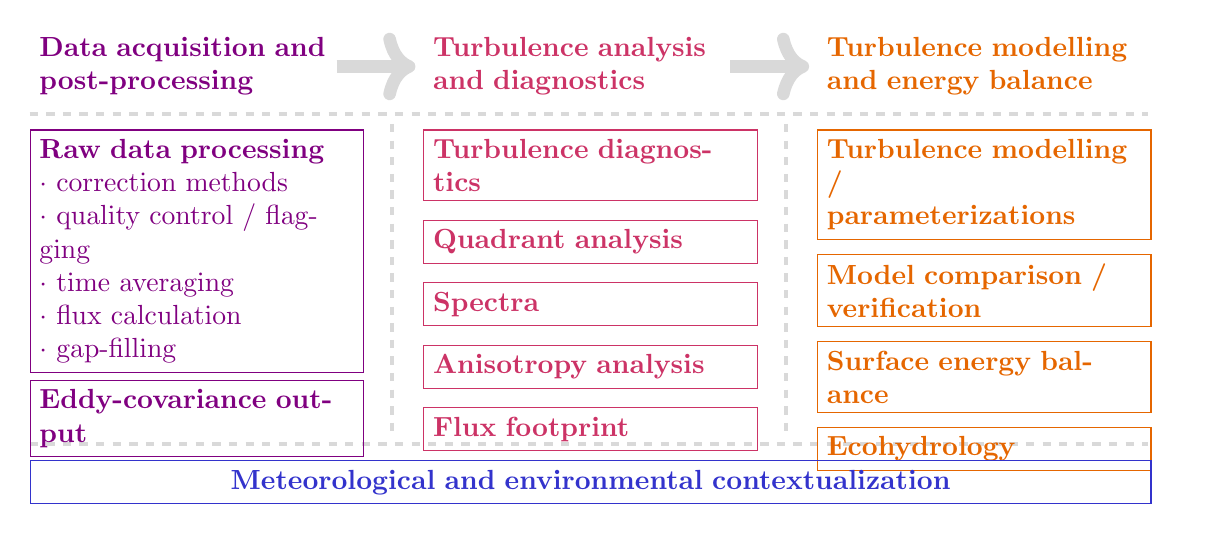
\begin{tikzpicture}
		\node(data) [text width = 4cm,lila,anchor=north west] at (0,0) { \textbf{Data acquisition and post-processing}} ;
		\node(analysis) [text width = 4cm, darkred,anchor=north west] at (5,0) { \textbf{Turbulence analysis \\ and diagnostics} };
		\node(application) [text width = 4.5cm,orange,anchor=north west] at (10,0) { \textbf{Turbulence modelling \\ and energy balance} };
		
		%----------------------------------------------------------------
		\draw [arrows = {-Computer Modern Rightarrow[line cap=round]},gray,line width=1.6mm]
		(3.9,-0.5) -- (4.9,-0.5);
		\draw [arrows = {-Computer Modern Rightarrow[line cap=round]},gray,line width=1.6mm]
		(8.9,-0.5) -- (9.9,-0.5);
		
		\draw [gray,line width=0.5mm,dashed]
		(4.6,-1.23) -- (4.6,-5.2);
		\draw [gray,line width=0.5mm,dashed]
		(9.6,-1.23) -- (9.6,-5.2);
		\draw [gray,line width=0.5mm,dashed]
		(0,-1.1) -- (14.2,-1.1);
		\draw [gray,line width=0.5mm,dashed]
		(0,-5.3) -- (14.2,-5.3);
		
		%--------------------------------------------------------------------
		\node(raw) [text width = 4cm,lila,draw,anchor=north west] at (0,-1.3) { \textbf{Raw data processing } \\
			$\cdot$ correction methods \\
			$\cdot$ quality control / flagging \\
			$\cdot$ time averaging \\
			$\cdot$ flux calculation \\
			$\cdot$ gap-filling
			
			%				$\cdot$ despiking \\
			%				$\cdot$ lag-time correction \\
			%				$\cdot$ detrending \\
			%				$\cdot$ coordinate rotation \\
			%				$\cdot$ time averaging $\rightarrow$ mean \\
			%				$\cdot$ calculation of covariances \\
			%				$\cdot$ WPL correction \\
			%				$\cdot$ SND correction \\
			%				$\cdot$ unit conversion $\rightarrow$ flux \\
			%				$\cdot$ quality flagging \\
			%				$\cdot$ flux gap-filling \\
			%				$\cdot$ spectral corrections
		} ;
		
		\node(download) [below=0.09cm of raw, text width = 4cm,lila,draw]  { \textbf{Eddy-covariance output} \\
			%				$\cdot$ from FLUXNET
		} ;
		
		
		%---------------------------------------------------------------------
		\node(diagnostics) [text width = 4cm,darkred,draw,anchor=north west]  at (5,-1.3) { \textbf{Turbulence diagnostics} \\
			%				$\cdot$ stability parameter \\
			%				$\cdot$ TKE, friction velocity, ...  
		} ;
		\node(qa) [text width = 4cm,darkred,draw,below=0.233cm of diagnostics] { \textbf{Quadrant analysis} \\
			%				$\cdot$ coherent structures \\
			%				$\cdot$ organization ratio 
		} ;
		\node(spectra) [text width = 4cm,darkred,draw,below=0.233cm of qa] { \textbf{Spectra} \\
			%				$\cdot$ averaged FFT spectra\\
			%				$\cdot$ MRD spectra / wavelets
		} ;
		\node(aniso) [text width = 4cm,darkred,draw,below=0.233cm of spectra] { \textbf{Anisotropy analysis} \\
			%				$\cdot$ Reynolds stress tensor\\
			%				%$\cdot$ turbulence anisotropy \\
			%				$\cdot$ barycentric map
		} ;
		\node(footprint) [text width = 4cm,darkred,draw,below=0.233cm of aniso] { \textbf{Flux footprint} \\
			%				$\cdot$ 2D flux footprint
		} ;
		
		%---------------------------------------------------------------
		
		\node(param) [text width = 4cm,orange,draw,anchor=north west]  at (10,-1.3) { \textbf{Turbulence modelling / \\ parameterizations} \\
			%				$\cdot$ bulk closures  \\
			%				$\cdot$ eddy-diffusivity closures \\
			%				$\cdot$ flux-variance relations \\  
			%				$\cdot$ flux-profile relations
		} ;
		\node(comp) [text width = 4cm,orange,draw,below=0.175cm of param] { \textbf{Model comparison / \\ verification\\}
			%				$\cdot$ model data processing 
		} ;
		\node(seb) [text width = 4cm,orange,draw,below=0.175cm of comp] { \textbf{Surface energy balance} \\
			%				$\cdot$ radiative fluxes \\
			%				$\cdot$ residual and closure ratio
		} ;
		\node(hyrdo) [text width = 4cm,orange,draw,below=0.175cm of seb] { \textbf{Ecohydrology} \\
			%				$\cdot$ Bowen ratio \\
			%				$\cdot$ evaporative fraction\\
			%				$\cdot$ flux partitioning
		} ;
		
		
		%----------------------------------------------------------
		\node(meteo) [text width = 14cm,madrid,anchor=north west,draw,align=center] at (0,-5.5) { \textbf{Meteorological and environmental contextualization} \\
			%				$\cdot$ wind speed profiles, gradients, Richardson number, clear-sky index, ...
		} ;
		
		
		%\draw[->, >=stealth',line width=1.5pt,text width=5cm, align=left] (start) -- (rans) node[midway,right] {\textbf{apply}: \\Reynolds average \\ Boussinesq approximation\\hydrostatic approximation} ;	
		
	\end{tikzpicture}
	\centering
	
\end{figure}






\end{document}